\chapter{Test mechanics}\label{sec:ch3}

In this chapter, we explain how to implement the lightweight proof of concept. The intention of the lightweight version is to know that the test approach is able to find bugs in generated systems. Therefore, we need to understand how the existing foundations from Rebel can be reused.

\info{lezen over: small world hypothesis}

\section{The account specification}
An extended account specification~\footnote{\url{https://github.com/cwi-swat/rebel/blob/e58590c7f51f59e7ee6443bb89ef09dff6febab6/rebel-core/examples/simple_transaction/Account.ebl}} from \autoref{fig:simple-account-spec} is used for this proof of concept, the implementation in Rebel is shown in \autoref{fig:account-spec}. According to the specification, an account can be opened with a minimum deposit of 50 euro. When an account is opened, it is possible to withdraw or deposit money. Besides deposit and withdraw, the balance may increase or decrease by interest. To disable any account, the block event can be used to put the account to the state blocked. The final state of account is closed, therefore there should not be any remaining balance. When an account is in the state closed, no further action is allowed since it is in the final state. The invariant is specified to keep every account with a positive balance.

% invariant paper ref, should be implemented in every event

\begin{sourcecode}[h!]
\begin{lstlisting}[]
specification Account {
	fields {
		accountNumber: IBAN @key
		balance: Money
	}

	events {
		openAccount[minimalDeposit = EUR 50.00]
		withdraw[]
		deposit[]
		interest[]
		block[]
		unblock[]
		close[]
	}

	invariants {
		positiveBalance
	}

	lifeCycle {
		initial init -> opened: openAccount

		opened -> opened: withdraw, deposit, interest
			     -> blocked: block
			     -> closed: close

		blocked -> opened: unblock

		final closed
	}
}
\end{lstlisting}
\caption{Account specification}\label{fig:account-spec}
\end{sourcecode}
\FloatBarrier

The specification of account has a close event\footnote{\url{https://github.com/cwi-swat/rebel/blob/e58590c7f51f59e7ee6443bb89ef09dff6febab6/rebel-core/examples/simple_transaction/Library.ebl}}
to close an account which is illustrated in \autoref{fig:account-close-event}.
The precondition of the close event is that the balance of the account should be
equal to zero. There are no postconditions, this means that the postconditions
are satisfied. So there are no properties changed of the account, but only the state
is changed to closed.

\begin{sourcecode}[h!]
\begin{lstlisting}[]
event close() {
	preconditions {
		this.balance == EUR 0.00;
	}
}
\end{lstlisting}
\caption{close event definition from account specification}\label{fig:account-close-event}
\end{sourcecode}
\FloatBarrier

\section{Introducing a bug}

As mentioned earlier, an initial lightweight version is expected, then it will be extended with motivated improvements with evaluation and validation. The approach is to start with a lightweight version which is able to trigger a bug and test it with the SMT Solver. For the lightweight version, it is an easily reproducible bug. This lightweight version is then able to trigger and test one specific bug.

\autoref{fig:account-close-pre} illustrates the code which is generated to check the precondition for the close event. From this code, we can see that the balance of an account should be zero before it is getting closed. We assume that the precondition is correctly generated.

\begin{sourcecode}[h!]
\begin{lstlisting}[language=scala]
case Close() => {

  checkPreCondition(({
    require(data.nonEmpty, s"data should be set, was: $data")
    require(data.get.balance.nonEmpty, s"data.get.balance should be set, was: $data.get.balance")
    data.get.balance.get
  } == EUR(0.00)), "this.balance == EUR 0.00")

}
\end{lstlisting}
\caption{Generated Precondition for close event}\label{fig:account-close-pre}
\end{sourcecode}
\FloatBarrier

The first bug to trigger is to close an account with some balance. In order to do this, the precondition of the close event should be changed in the generated system (see \autoref{fig:mod-spec-gen}). By manually making the changes in the generated system (system under test), we know that there is definitely a bug in the generated system, assuming that the specification is correct.

The modified precondition looks as follows in \autoref{fig:account-close-mod-pre}. The precondition is changed to \textit{RebelConditionCheck.success}, this means that the precondition is satisfied.

\begin{figure}[h!]
  \centering
  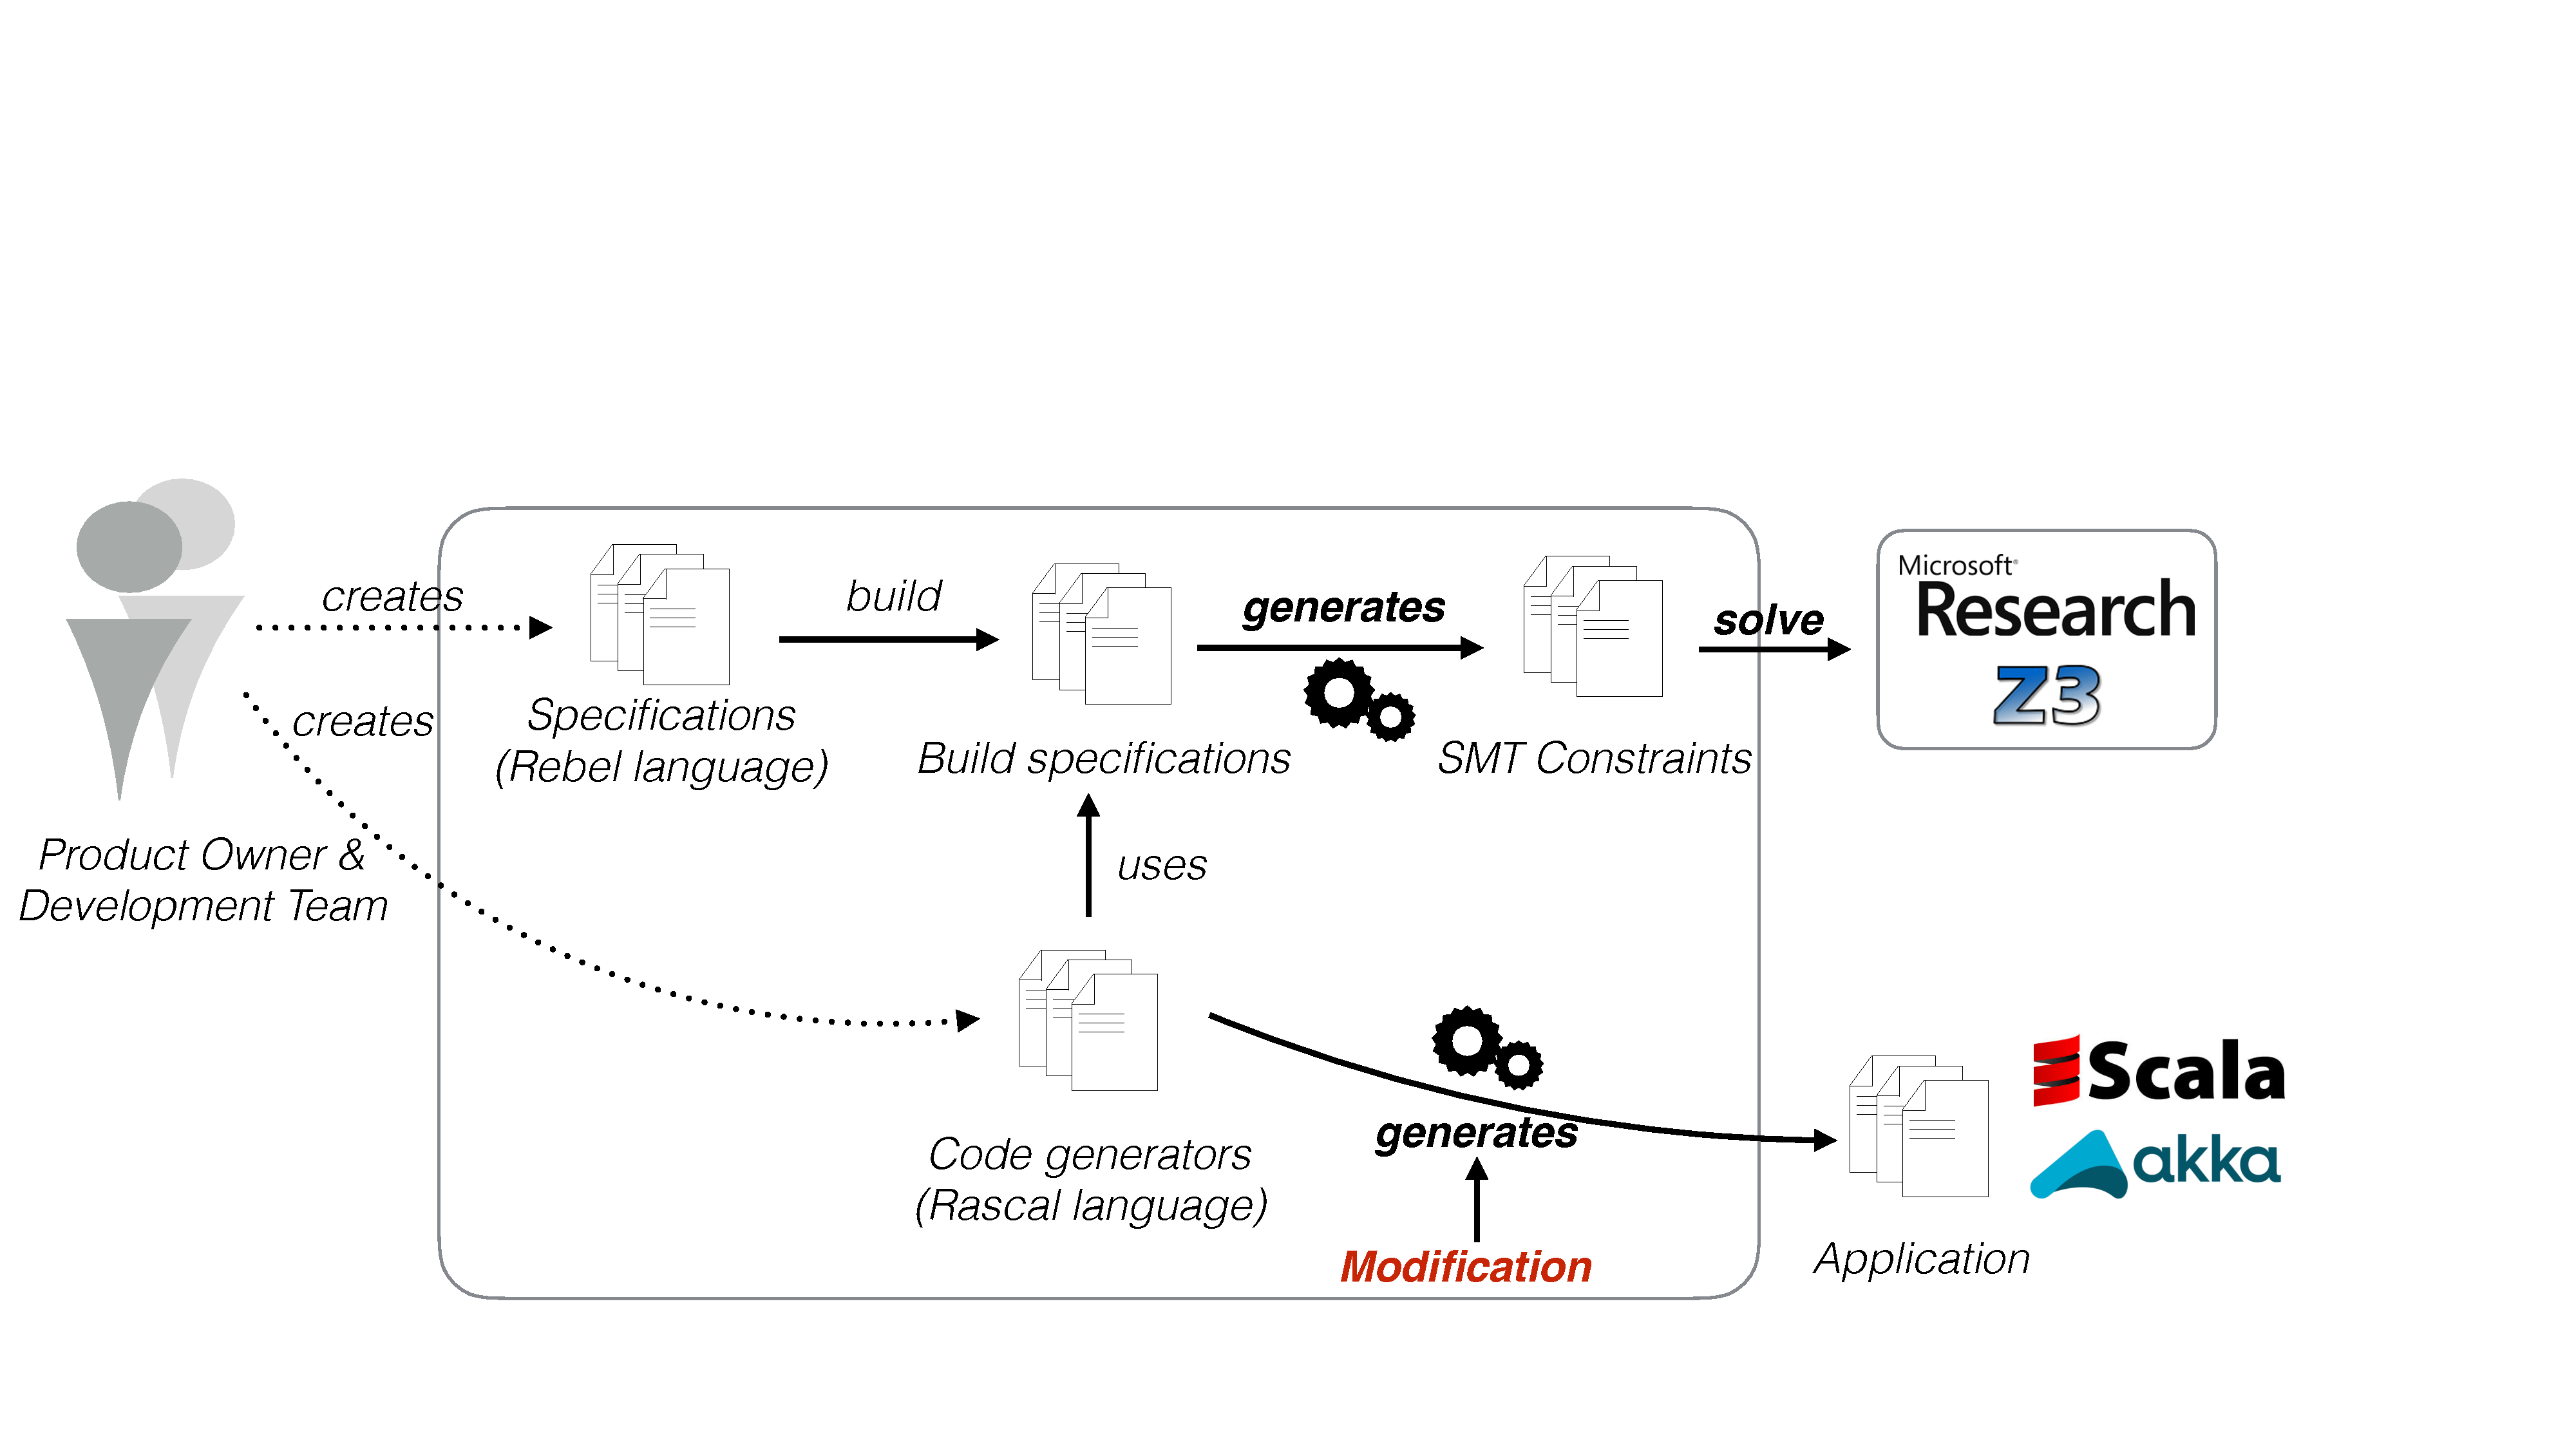
\includegraphics[scale=0.26]{figures/mod-generated.pdf}
  \caption{Modification in specification development}\label{fig:mod-spec-gen}
\end{figure}
\FloatBarrier

\begin{sourcecode}[h!]
\begin{lstlisting}[language=scala]
case Close() => {
  RebelConditionCheck.success
}
\end{lstlisting}
\caption{Modified Precondition for close event}\label{fig:account-close-mod-pre}
\end{sourcecode}
\FloatBarrier

Right now we have introduced a bug in the system under test (SUT), so the
generated system doesn't conform to the specification. We discussed earlier that
we are going to use the SMT solver to find bugs in the SUT.

Having an account with some balance in the state closed should not be possible
according to the specification. To let the SMT Solver solve this situation, it
is necessary to generate the appropriate SMT formulas. Therefore, checking can
be used to check whether the given state with its properties is reachable.

For this situation, is the following tebl file created, which is shown in
\autoref{fig:tebl-closed-account}. It defines the state of a closed account with
the property balance, where the balance isn't equal to zero. Also, here is 6
used as configurable time-out. The SMT solver tries to solve this problem in
max 6 steps.

\begin{sourcecode}[h!]
\begin{lstlisting}[]
module simple_transaction.ClosedAccountWithBalance

import simple_transaction.Account

state closedAccountWithBalance {
  closed Account with balance != EUR 0.00;
}

check closedAccountWithBalance reachable in max 6 steps;
\end{lstlisting}
\caption{Closed account test}\label{fig:tebl-closed-account}
\end{sourcecode}
\FloatBarrier

The input for the SMT solver is now defined. Similar behaviour should be defined
for the generated system. So an account needs to be opened and closed
afterwards.

The tebl file is passed to the model checker and it returns whether the given
SMT problem is reachable or not. A state is reachable when it can be reached
from the initial state via valid
transitions.~\cite[p.~4]{stoel_storm_vinju_bosman_2016} To check if the state is
reachable in the generated system, the request made for the given transition
contains afterwards a check whether the request is successful.

Since we've defined the input for both systems and are able to compare it, we
can trigger the bug and compare the results of it. As you can see in
\autoref{fig:result-trigger-one-bug}, the results of the model checker state
that the defined state in \autoref{fig:tebl-closed-account} isn't reachable and
that the state in the SUT is reachable.

\begin{sourcecode}[h!]
\begin{lstlisting}[]
rascal>check()

Reachable state false
Closed account true
bool: false
\end{lstlisting}
\caption{Results closing account comparison}\label{fig:result-trigger-one-bug}
\end{sourcecode}
\FloatBarrier

\section{Evaluation}\label{sec:ch3-evalution}
As we have seen with this lightweight version, it is able to find one specific bug with the use of an SMT Solver. Since the code generator is template based, it is possible to find faults in templating. There are two parts where there can occur faults during the generation parts. As first,~\cite[p.274]{voelter2013dsl} states that a majority of the generated code is fixed, some isolated parts are dependent on the input of the model. So it is possible that there might be bugs in the fixed code (skeleton). The second part is the template control code which is injected into the generated code. The manually introduced bug from the previous chapter belongs  to this category.

\unsure{\textbf{Onduidelijkheid DSL fowler}: styles of code generation: Model-Aware Generation and Model Ignorant Generation. Styles for generating textual output: Transformer
Generation and Templated Generation.}

\info{transactions, atomic commits, consistency. <- dit is moeilijk te doen. welke bugs verwacht je? het is moeilijk iets te generate. en uitleggen waarom het moeilijk is testen.}
